% Poster — Language-Reasoning Interference via SAEs
% Compile with: pdflatex poster.tex (or upload to Overleaf)
% Uses tikzposter for clean academic poster layout
\documentclass[25pt, a0paper, landscape]{tikzposter}

\usepackage[T1]{fontenc}
\usepackage{amsmath, amssymb}
\usepackage{booktabs}
\usepackage{microtype}
\usepackage{graphicx}
\usepackage{xcolor}
\usepackage{enumitem}
\usepackage{multicol}

% ---------- Theme ----------
\usetheme{Default}
\usecolorstyle{Denmark}

% Custom colors
\definecolor{MITred}{HTML}{A31F34}
\definecolor{darkblue}{HTML}{1a365d}
\definecolor{accentblue}{HTML}{2563eb}
\definecolor{lightgray}{HTML}{f5f5f5}
\definecolor{gain}{HTML}{27ae60}
\definecolor{loss}{HTML}{c0392b}

\definecolorstyle{MITStyle}{
  \definecolor{colorOne}{HTML}{1a365d}
  \definecolor{colorTwo}{HTML}{2563eb}
  \definecolor{colorThree}{HTML}{A31F34}
}{
  \colorlet{backgroundcolor}{white}
  \colorlet{framecolor}{colorOne}
  \colorlet{titlefgcolor}{white}
  \colorlet{titlebgcolor}{colorOne}
  \colorlet{blocktitlebgcolor}{colorOne}
  \colorlet{blocktitlefgcolor}{white}
  \colorlet{blockbodybgcolor}{white}
  \colorlet{blockbodyfgcolor}{black}
}
\usecolorstyle{MITStyle}

% Compact lists
\setlist[itemize]{leftmargin=1.2em, itemsep=0.2em, topsep=0.2em}
\setlist[enumerate]{leftmargin=1.5em, itemsep=0.2em, topsep=0.2em}

% ---------- Title ----------
\title{\parbox{0.95\linewidth}{\centering
  From Subspaces to Features: Causal Feature Profiling of\\[0.15em]
  Language-Reasoning Interference in Multilingual LLMs}}
\author{Karlo Vrancic, Anastasia Ahani, Riley Kong}
\institute{MIT 6.8610 --- Quantitative Methods for Natural Language Processing --- Spring 2026}

\begin{document}

\maketitle[width=0.98\textwidth]

% ===================================================================
% ROW 1
% ===================================================================
\begin{columns}

% ------------------------------------------------------------------
% PANEL 1: Motivation & Setup
% ------------------------------------------------------------------
\column{0.32}
\block{1. Motivation \& Setup}{

\textbf{Problem.}
Multilingual LLMs reason worse in non-English languages.
Zhao et al.\ (NeurIPS 2025) showed that removing language subspaces via SVD
improves multilingual reasoning --- but their method is coarse (operates on
entire subspaces) and cannot explain why the effect varies across languages.

\textbf{Our approach.}
We use \textbf{Sparse Autoencoders} (Gemma Scope 2) for
\emph{per-feature} decomposition of the residual stream, enabling:
\begin{itemize}
  \item Individual feature identification (monolinguality + probe)
  \item Individual feature ablation with causal measurement
  \item Per-language, per-feature mechanistic analysis
\end{itemize}

\textbf{Setup.}
\begin{itemize}
  \item \textbf{Model:} Gemma 3 4B IT (34 layers, $d_\text{model}=2560$, BF16)
  \item \textbf{SAEs:} 16k-width residual SAEs at layers \{9, 17, 22, 29\}
  \item \textbf{Data:} MGSM --- 250 math problems $\times$ 5 languages (en, zh, es, bn, sw)
  \item \textbf{Feature ID:} Method A (monolinguality $\nu$) $\cap$
        Method B (supervised probe) $\to$ candidate features
  \item \textbf{Probe ceiling:} 0.88 across all layers --- language identity is mostly
        but not perfectly linearly decodable in SAE feature space
\end{itemize}

\vspace{0.3em}
\textbf{Three feature identification methods.}
Following prof's guidance (``use 3 methods; disagreement is a finding''):
\begin{enumerate}
  \item \textbf{A --- Monolinguality:} $\nu_s^L = \mu_s^L - \gamma_s^L$
  \item \textbf{B --- Supervised probe:} LogisticRegression on SAE features
  \item \textbf{C --- Cross-lingual reasoning:} features active across all 5 langs
\end{enumerate}
A$\cap$B intersection selects candidates; C identifies reasoning features.

%% Small probe-accuracy figure placeholder
%\begin{center}
%\includegraphics[width=0.9\linewidth]{figures/paper_fig2_phase1.png}
%\end{center}
}

% ------------------------------------------------------------------
% PANEL 2: Main Result --- SAE ablation vs Zhao
% ------------------------------------------------------------------
\column{0.36}
\block{2. SAE Ablation vs.\ Zhao SVD Baseline}{

Ablate top-$k$ A$\cap$B features per language at layer 17 using
directional (QR-orthogonalized) projection.
Best $k=20$ selected on 50-prompt dev split.

\vspace{0.5em}

\begin{center}
\renewcommand{\arraystretch}{1.15}
\begin{tabular}{l c c c c}
\toprule
\textbf{Lang} & \textbf{Baseline} & \textbf{Zhao SVD} & \textbf{SAE $k$=20}
  & \textbf{$\Delta$ vs base} \\
\midrule
en & 0.580 & 0.632 & \textbf{\textcolor{gain}{0.712}} & \textbf{\textcolor{gain}{+13.2pp}} \\
es & 0.568 & 0.600 & \textbf{\textcolor{gain}{0.636}} & \textbf{\textcolor{gain}{+6.8pp}} \\
zh & 0.624 & 0.624 & 0.596 & $-$2.8pp \\
sw & 0.320 & 0.332 & 0.296 & $-$2.4pp \\
bn & 0.564 & 0.564 & \textcolor{loss}{0.480} & \textbf{\textcolor{loss}{$-$8.4pp}} \\
\midrule
\textbf{avg} & 0.531 & 0.550 & 0.544 & +1.3pp \\
\bottomrule
\end{tabular}
\end{center}

\vspace{0.3em}

\textbf{Key finding:} the per-language pattern is sharp and predictable.

\begin{itemize}
  \item \textbf{en} (+13.2pp) and \textbf{bn} ($-$8.4pp) are both statistically
        significant (non-overlapping bootstrap 95\% CIs at $n=250$).
  \item The pattern correlates with \emph{feature profile}: per-feature ablation
        shows en's top features affect \emph{only} perplexity (clean language features),
        while bn's features affect \emph{both} perplexity and accuracy (entangled).
  \item \textbf{ppl-$\Delta$ $\times$ acc-$\Delta$ scatter} (right) visualizes this:
        en clusters in the ``language-only'' zone; bn in the ``shared'' zone.
\end{itemize}

\vspace{0.3em}
\textbf{Supporting results:}
\begin{itemize}
  \item \textbf{Language fidelity:} SAE preserves output language better than
        Zhao for en (+3.2pp) and es (+4.8pp); bn drops ($-$12.8pp) --- predicted
        by its entangled profile
  \item \textbf{Layer dependence:} inverted-U peaking at L22 (+6.1pp avg).
        L29 ablation hurts ($-$5.5pp) --- late-layer features are too entangled
  \item \textbf{Controls:} random feature ablation $=$ no signal;
        Deng-only (Method A) does better on en but worse on bn
\end{itemize}
}

% ------------------------------------------------------------------
% PANEL 3: Mechanism --- Capacity Competition
% ------------------------------------------------------------------
\column{0.32}
\block{3. Mechanism: Capacity Competition}{

\textbf{Setup.} Ablate top-20 language features at L17, measure activation
change of 21 candidate reasoning features (forward-only, 50 problems $\times$
5 langs). Wilcoxon signed-rank test per (lang, feature).

\vspace{0.5em}

\textbf{Headline:} ablating language features \textbf{releases dormant
reasoning features}.

\begin{center}
\renewcommand{\arraystretch}{1.1}
\begin{tabular}{l r r r r}
\toprule
\textbf{Lang} & \textbf{Feature} & \textbf{Clean} & \textbf{Ablated} & \textbf{$\Delta$} \\
\midrule
sw & 96 & 0 & 7036 & \textcolor{gain}{+7036} \\
es & 96 & 0 & 2856 & \textcolor{gain}{+2856} \\
en & 96 & 0 & 2577 & \textcolor{gain}{+2577} \\
zh & 96 & 0 & 2501 & \textcolor{gain}{+2501} \\
bn & 96 & 0 & 2345 & \textcolor{gain}{+2345} \\
\midrule
en & 34 & 2177 & 0 & \textcolor{loss}{$-$2177} \\
\bottomrule
\end{tabular}
\end{center}
\vspace{0.2em}
{\small All $p < 1.8 \times 10^{-15}$ (Wilcoxon).}

\vspace{0.5em}

\textbf{Two patterns:}
\begin{enumerate}
  \item \textbf{Dormant $\to$ active:} Feature 96 has zero activation normally
        but explodes to 2345--7036 across all 5 languages when language features
        are removed. These are \emph{released} reasoning features.
  \item \textbf{Active $\to$ suppressed:} Feature 34 collapses from $\sim$2177
        to 0 --- representational space gets reclaimed.
\end{enumerate}

\textbf{Direct evidence:} language and reasoning features \emph{compete for
residual-stream capacity}. Removing language features doesn't just turn off
language outputs --- it actively releases dormant reasoning features.

\vspace{0.3em}
\textbf{Downstream cascade:}
\begin{itemize}
  \item L17 ablation propagates to L29: Swahili's top monolinguality feature
        (f8612, $\nu=5293$) shifts by $|\Delta|=6896$
  \item Attention entropy reorganizes at L22/L29 (significant in 4/5 languages)
  \item en/bn: attention becomes more \emph{peaked} (focused);
        es/sw: more \emph{spread} (uncertain)
\end{itemize}
}

\end{columns}

% ===================================================================
% ROW 2
% ===================================================================
\begin{columns}

% ------------------------------------------------------------------
% PANEL 4: Per-feature ablation scatter (supporting, de-emphasized)
% ------------------------------------------------------------------
\column{0.25}
\block{4. Per-Feature Ablation Profile}{

Individual ablation of top-5 A$\cap$B candidates per language at L17.
Each feature measured on perplexity-$\Delta$ (language disruption) and
accuracy-$\Delta$ (reasoning disruption).

\vspace{0.3em}

\begin{center}
\renewcommand{\arraystretch}{1.1}
{\small
\begin{tabular}{l r r r r}
\toprule
\textbf{Lang} & \textbf{Lang-only} & \textbf{Shared} & \textbf{Reas.} & \textbf{Junk} \\
\midrule
en & \textbf{5} & 0 & 0 & 0 \\
es & \textbf{3} & 0 & 1 & 1 \\
zh & 3 & 2 & 0 & 0 \\
sw & 2 & \textbf{3} & 0 & 0 \\
bn & 0 & \textbf{5} & 0 & 0 \\
\bottomrule
\end{tabular}
}
\end{center}

\vspace{0.3em}

The degree of language--reasoning entanglement \textbf{varies sharply across
languages}: English has cleanly separable language features (all 5 affect
only perplexity); Bengali has none (all 5 also affect accuracy).

\vspace{0.2em}

This per-feature profile \emph{predicts} the group ablation outcome in Panel 2:
more clean language features $\to$ bigger accuracy gain.

%% Scatter plot placeholder
%\begin{center}
%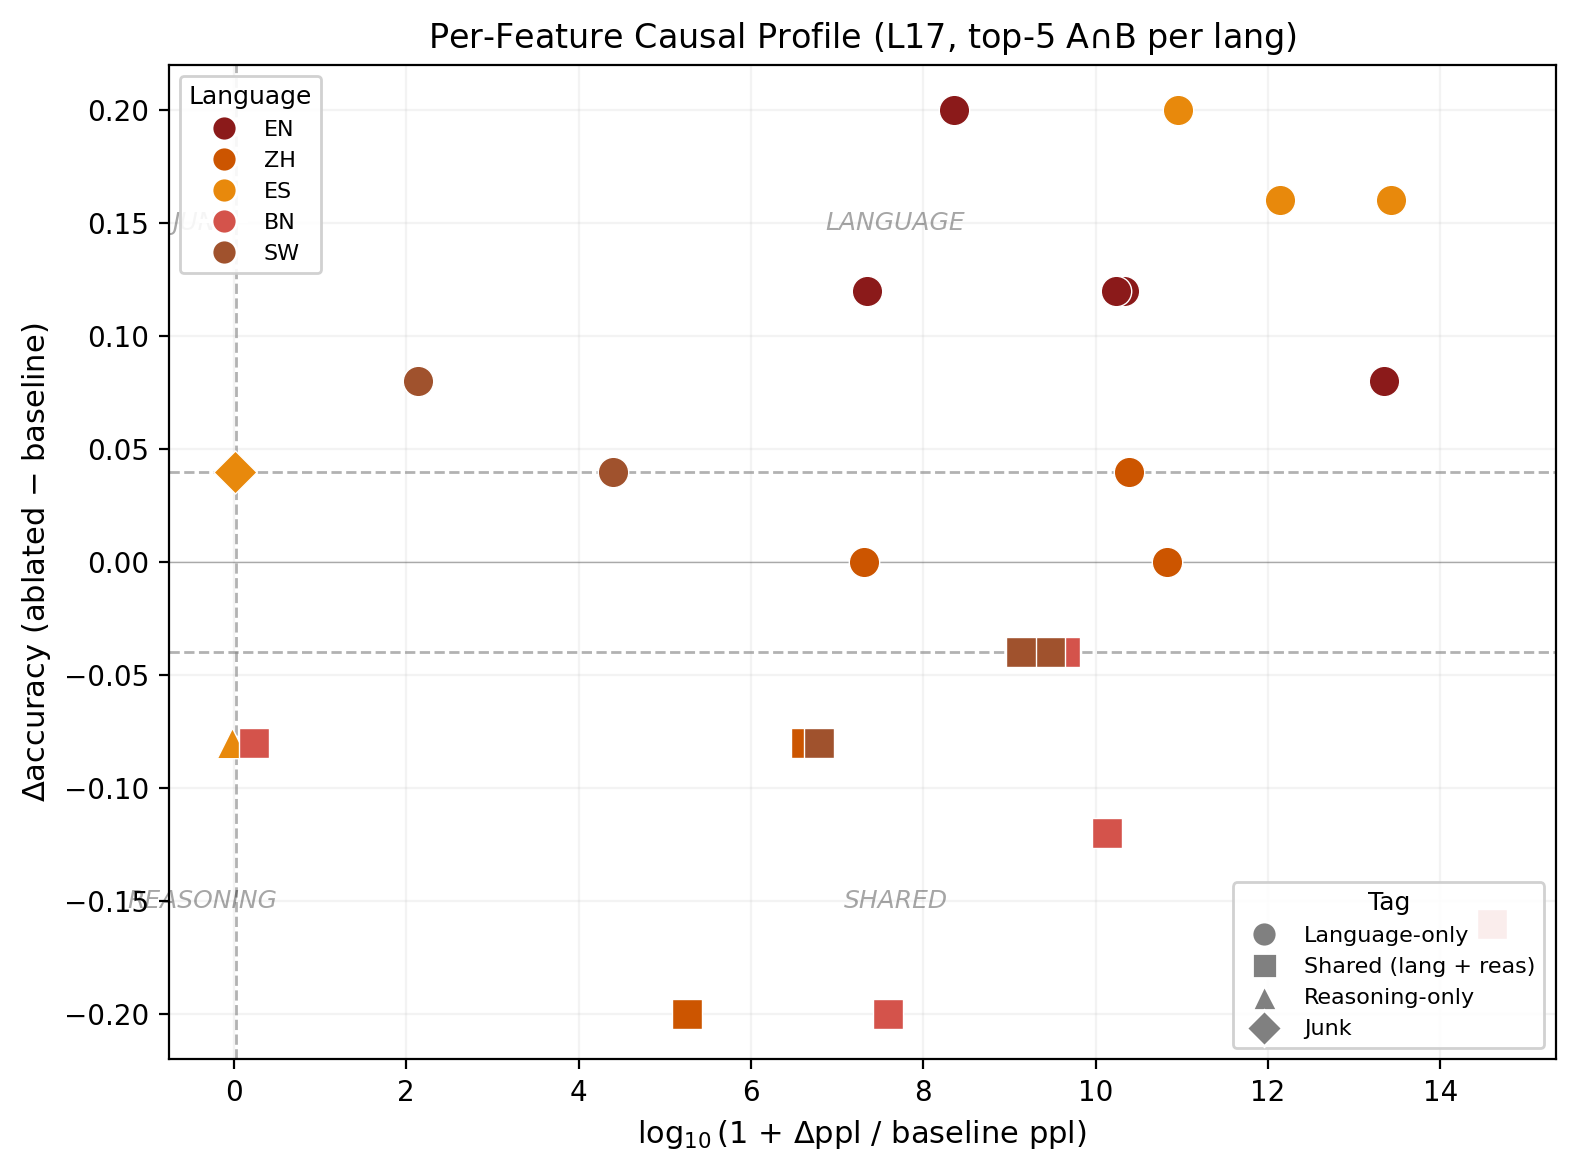
\includegraphics[width=0.85\linewidth]{figures/ppl_acc_scatter.png}
%\end{center}
}

% ------------------------------------------------------------------
% PANEL 5: The Twist --- FLORES generalization failure
% ------------------------------------------------------------------
\column{0.42}
\block{5. The Features Don't Generalize Out-of-Domain}{

The per-feature profiles predict MGSM outcomes. \textbf{But are these features
really encoding \emph{language}?} We test on FLORES-200 (1012 parallel
translations, content held constant across languages).

\vspace{0.5em}

\begin{center}
\renewcommand{\arraystretch}{1.15}
\begin{tabular}{l c c c c c}
\toprule
\textbf{Metric} & \textbf{en} & \textbf{zh} & \textbf{es} & \textbf{bn} & \textbf{sw} \\
\midrule
$\nu$ correlation (MGSM$\leftrightarrow$FLORES) &
  \textcolor{gain}{0.76~\checkmark} & \textcolor{gain}{0.73~\checkmark} &
  \textcolor{loss}{0.23~\texttimes} & \textcolor{loss}{$-$0.21~\texttimes} &
  \textcolor{gain}{0.88~\checkmark} \\
Target activation ratio &
  \textcolor{gain}{2.0x~\checkmark} & \textcolor{gain}{6.2x~\checkmark} &
  \textcolor{loss}{1.4x~\texttimes} & \textcolor{gain}{5.4x~\checkmark} &
  \textcolor{gain}{6.7x~\checkmark} \\
\bottomrule
\end{tabular}
\end{center}

\vspace{0.3em}

\begin{minipage}[t]{0.48\linewidth}
\textbf{Global metrics (all fail):}
\begin{itemize}
  \item Probe transfer (MGSM$\to$FLORES): \textcolor{loss}{\textbf{0.714}} (need $>$0.80)
  \item Language-only vs Shared separation: \textcolor{loss}{$p=0.51$} (need $<$0.01)
  \item Monolinguality correlation: 3/5 pass, 2/5 fail
\end{itemize}
\end{minipage}
\hfill
\begin{minipage}[t]{0.48\linewidth}
\textbf{What this means:}
\begin{itemize}
  \item The per-feature profiles are an \textbf{effective in-domain prediction tool}
        (they predict intervention outcomes on MGSM)
  \item But the underlying features are \textbf{not stable, general-purpose
        language encodings}
  \item The interference is \textbf{partially domain-specific} --- tied to how
        language interacts with \emph{this particular task}
\end{itemize}
\end{minipage}

\vspace{0.5em}

\textbf{New experiment --- FLORES-derived feature ablation:}
\begin{enumerate}
  \item Run Phase 1 methods on FLORES activations $\to$ find ``general language
        features'' (domain-independent)
  \item Ablate those features on MGSM math problems
  \item Compare to MGSM-derived feature ablation
\end{enumerate}
If FLORES-derived features also improve reasoning when ablated $\to$ the
interference is from general language encoding. If only MGSM-derived features
help $\to$ the interference is domain-specific. \emph{(Results TBD --- experiment
in notebook 09.)}
}

% ------------------------------------------------------------------
% PANEL 6: Takeaways
% ------------------------------------------------------------------
\column{0.33}
\block{6. Takeaways \& Limitations}{

\textbf{Main findings:}

\begin{enumerate}
  \item \textbf{Per-feature ablation profiles predict intervention outcomes.}
        Individual ppl-$\Delta$ $\times$ acc-$\Delta$ measurements predict whether
        group ablation helps or hurts, per language.

  \item \textbf{English has cleanly separable language features; Bengali doesn't.}
        The degree of language--reasoning entanglement varies sharply across
        languages. This explains asymmetric results from Zhao et al.

  \item \textbf{Capacity competition is the mechanism.}
        Removing language features releases dormant reasoning features
        ($\Delta$ up to +7036, $p < 10^{-15}$), with cascading effects
        through L22 and L29.

  \item \textbf{In-domain features don't generalize out-of-domain.}
        FLORES validation shows the features are partially task-specific,
        not purely language-encoding.
\end{enumerate}

\vspace{0.5em}

\textbf{Limitations:}
\begin{itemize}
  \item Single model (Gemma 3 4B IT), single task (MGSM), 5 languages
  \item Dev/test overlap in profiling step (top-5 selected on 25 problems)
  \item FLORES-derived ablation experiment pending
  \item Global $k=20$ is suboptimal --- per-language $k$ selection
        would likely improve zh/sw/bn results
\end{itemize}

\vspace{0.5em}

\textbf{References:}
\begin{itemize}[itemsep=0.1em]
  \item Zhao et al.\ (NeurIPS 2025) --- Language subspace removal via SVD
  \item Deng et al.\ (2025) --- Monolinguality metric for SAE features
  \item Bricken et al.\ (2023) --- Sparse autoencoders for mechanistic interp.
  \item Lieberum et al.\ (2024) --- Gemma Scope SAE release
\end{itemize}

\vspace{0.5em}

{\small\textcolor{gray}{Code: \texttt{github.com/kvrancic/nlp-project}}}
}

\end{columns}

\end{document}
